\chapter{Diseño e implementación} % Main chapter title

\label{Chapter3} 
En este capítulo se realiza una explicación de la solución propuesta , el diseño de los circuitos impresos, el diseño del firmware y el diseño de la lógica programable.

\section{ Arquitectura de la solución propuesta}
Para cumplir los requerimientos enumerados en el capítulo \ref{Chapter2} se desarrolló la solución mostrada en la figura \ref{fig:solución}. Se utilizó la BOARD DE1-SoC en la cual se utilizó el FPGA para controlar la matriz de LEDs y el procesador para administrar el despliegue de las imagenes y manejar las comunicaciones con la estación remota.
\begin{figure}[htpb]
	\centering
	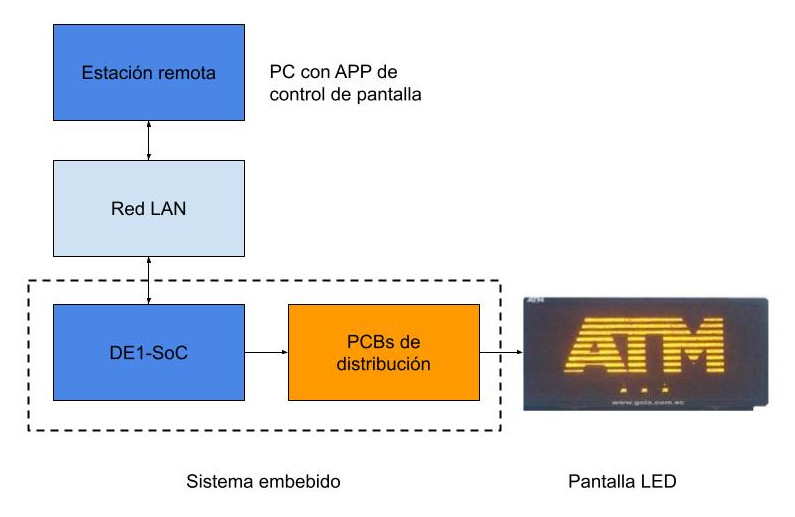
\includegraphics[scale=2]{Figures/Diagramasistemavms.jpg} 
	\caption{Esquema de la solución propuesta.}
	\label{fig:solución}
\end{figure}

En la figura \ref{fig:bloques embebido} se muestra el diagrama de bloques del sistema embebido. En la figura \ref{fig:bloques embebido} se muestra la interacción interna y externa de la BOARD DE1-SoC.
 
\begin{figure}[htpb]
	\centering
	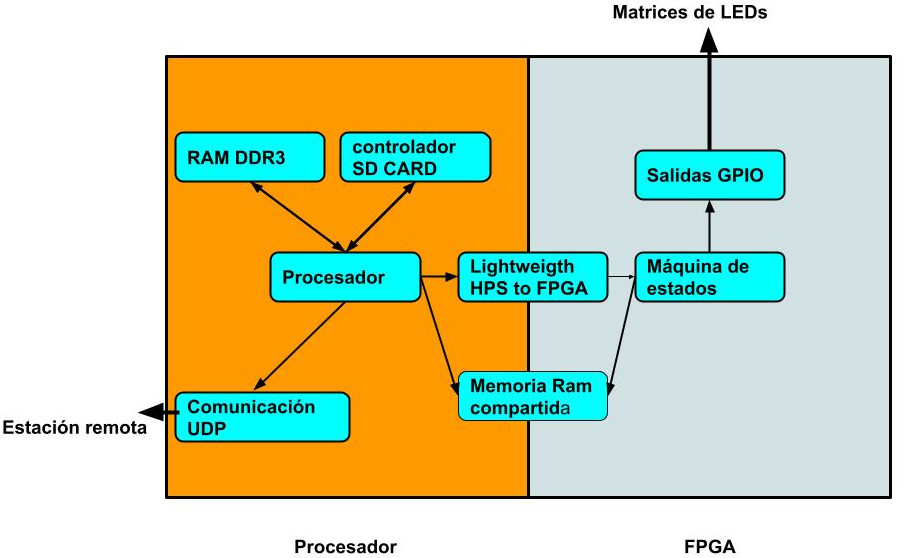
\includegraphics[scale=1.8]{Figures/Diagramabloques.jpg} 
	\caption{Diagrama de bloques del sistema embebido.}
	\label{fig:bloques embebido}
\end{figure}






\section{ Diseño de circuitos impresos}
Se diseñaron dos circuitos impresos (en inglés, PCB, Printed Circuit Board) para la construcción de la pantalla, una PCB matriz de LEDs y una PCB para distribuir señales de control desde el FPGA hacia las matrices de LEDs.
\subsection{PCB matriz de LEDs}
Para construir la pantalla LED se utilizaron varias PCBs matrices de LEDs. La PCB matriz LEDs tiene una resolución de 16 LEDs de ancho por 16 LEDS de largo. Los LED tienen un \textit{pitch} P-20. Se utilizó el conector IDC-16 para recibir y transmitir las señales de control. En la figura \ref{fig:pcbrenderfront}  se muestra la PCB desde una perspectiva frontal. En la figura \ref{fig:pcbrenderback} se muestra el lado posterior de la PCB.


\begin{figure}[htpb]
	\centering
	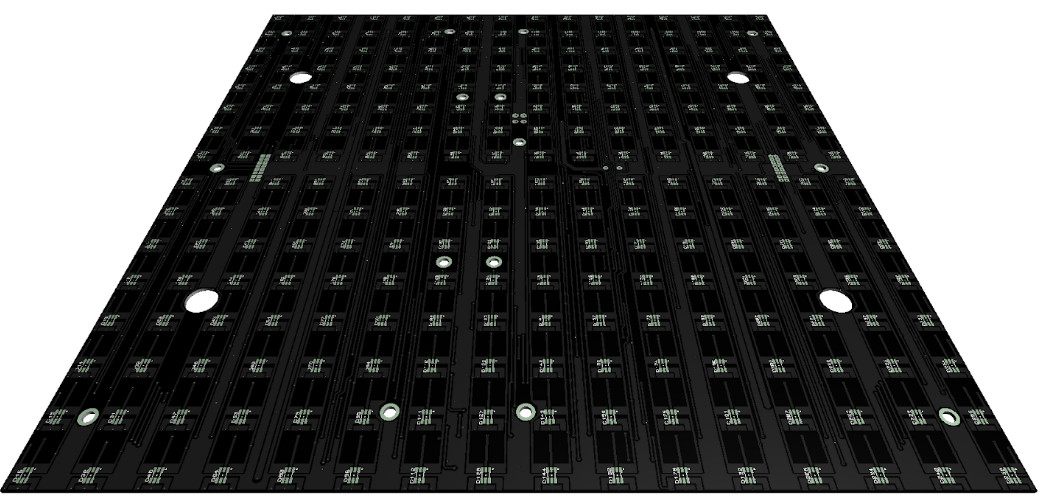
\includegraphics[scale=0.3]{Figures/pcbfullcolorfrontrender.jpg} 
	\caption{Vista frontal del PCB matriz de LEDs.}
	\label{fig:pcbrenderfront}
\end{figure}
\begin{figure}[htpb]
	\centering
	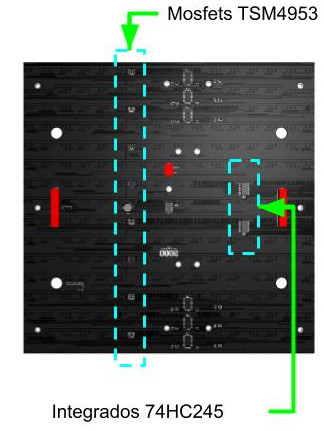
\includegraphics[scale=4]{Figures/pcbfullcolorbackrender.jpg} 
	\caption{Vista posterior del PCB matriz de LEDs.}
	\label{fig:pcbrenderback}
\end{figure}

En el diseño de la matriz de LEDs se usaron seis drivers de LEDs. Se necesitan tres drivers de LEDs para controlar un grupo de 8 filas por 16 columnas de LEDs. Cada driver habilita un solo color básico. En la figura \ref{fig:circuitombi} se muestra el circuito de conexión de uno de los drivers de LEDs. La resistencia R3 junto con el capacitor C17 forman un filtro pasa bajos. El inductor L5 protege al driver de la corriente que se producen cuando se desconecta la fila LEDs durante el barrido. 

\begin{figure}[htpb]
	\centering
    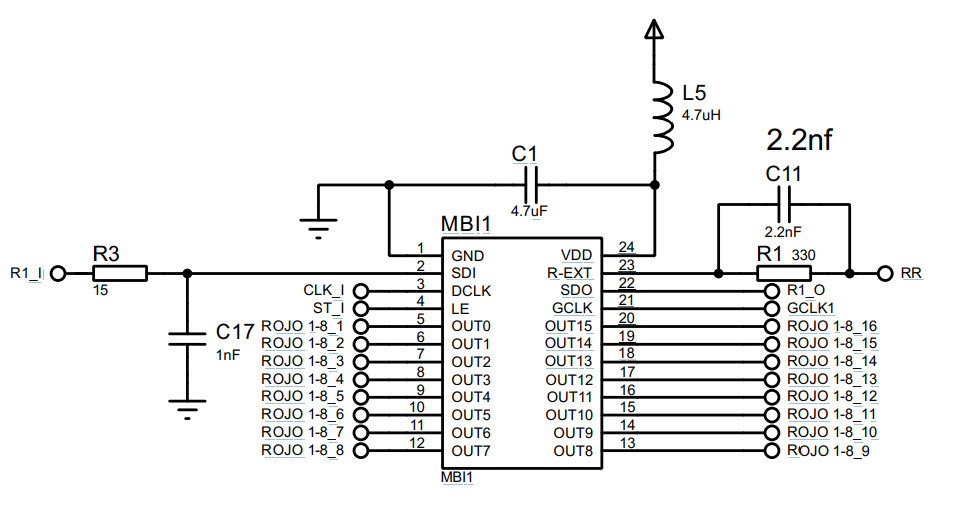
\includegraphics[scale=0.4]{Figures/circuitombi.jpg} 
	\caption{Esquemático de conexión de un MBI.}
	\label{fig:circuitombi}
\end{figure}



Como se explicó en el capítulo \ref{Chapter2} las filas son controladas por MOSFETs y las columnas son controladas mediante el driver MBI5051. En el circuito \ref{fig:circuitobarrido} se muestra el circuito de barrido. Las filas son habilitadas usando MOSFETs los cuales son controlados por el demultiplexor 74HC138. El funcionamiento del circuito se describe en la tabla \ref{tab:funcionamientobarrido}.

\begin{figure}[htpb]
	\centering
    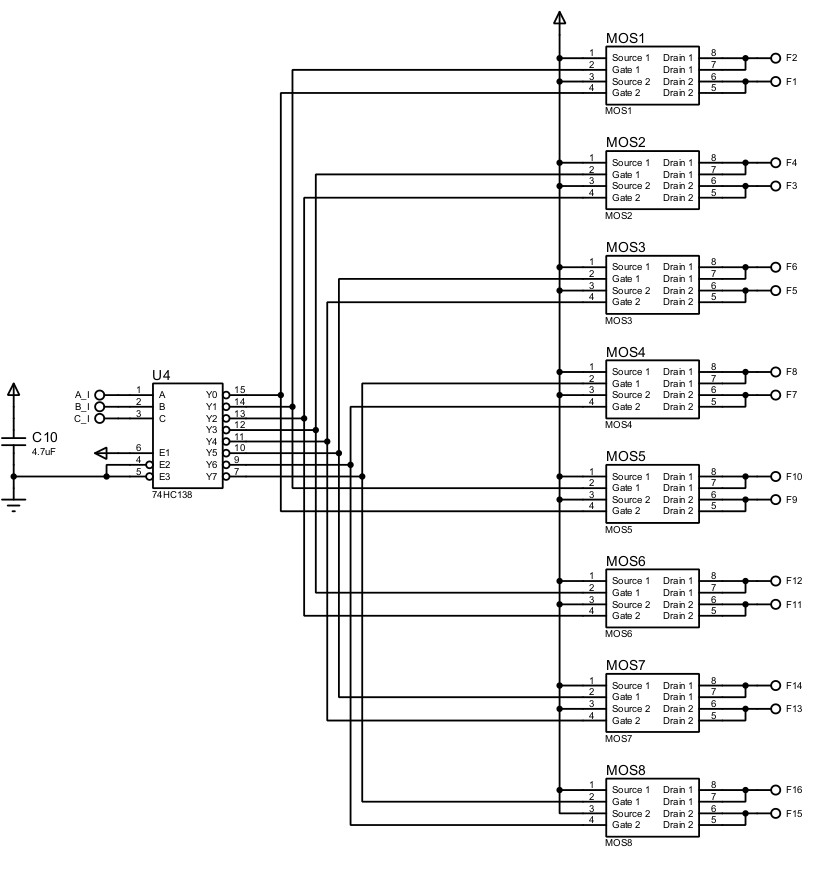
\includegraphics[scale=0.6]{Figures/circuitoBarrido.jpg} 
	\caption{Esquemático del circuito de barrido.}
	\label{fig:circuitobarrido}
\end{figure}


\begin{table}[h]
\centering
\caption[Funcionamiento circuito barrido]{Funcionamiento del circuito de barrido.}
\begin{tabular}{l c c c c}
\toprule
\textbf{A}& \textbf{B} & \textbf{C} & \textbf{Fila habilitada}\\
\midrule 


F &F &F &Fila F1 y Fila F9\\
T &F &F &Fila F2 y Fila F10\\
F &T &F &Fila F3 y Fila F11\\
T &T &F &Fila F4 y Fila F12\\
F &F &T &Fila F5 y Fila F13\\
T &F &T &Fila F6 y Fila F14\\
F &T &T &Fila F7 y Fila F15\\
T &T &T &Fila F8 y Fila F16\\


\bottomrule
\hline
\end{tabular}
\label{tab:funcionamientobarrido}
\end{table}


La figura \ref{fig:fotomatrixled} se muestra la PCB ensamblada. Esta PCB fue ensamblada en la empresa utilizando una maquina de \textit{pick and place}. La PCB fue soldada con un horno de soldadura para componentes de montaje superficial (Surface Mount Device, SMD). La curva de temperatura del horno se ajustó de acuerdo a las hojas de datos de el LED ya que esté es el elemento crítico.

\begin{figure}[htpb]
	\centering
    \includegraphics[scale=0.09]{Figures/frontmatrix.jpg} 
	\caption{Foto PCB matriz de LEDs.}
	\label{fig:fotomatrixled}
\end{figure}



\subsection{PCB de distribución}
La PCB de distribución cumple dos funciones. La primera función es elevar el voltaje de las señales de salida del FPGA y la segunda es distribuir la señal hacia las matrices de LEDs. En la figura \ref{fig:circuitodistribucion} se puede observar el esquemático que se utilizó para distribuir las señales desde el FPGA hacia las matrices de LEDs. 

En la figura \ref{fig:pcbrenderdistribuccionfrontal}  se muestra la PCB de distribución desde una perspectiva frontal. En la figura \ref{fig:circuitodistribucion} se muestra el circuito de una de las tres salidas de la PCB de distribución. Las señales de control que ingresan en el conector de cuarenta pines tienen un voltaje de 3,3 V mediante el integrado 74LVC245 en cual eleva el voltaje a 5 V. El cambio de nivel de voltaje es necesario debido a que las GPIOs de la BOARD DE1-SoC tienen un nivel de voltaje de 3,3 V y las matrices de LEDs funcionan con señales de control TTL. Para construir la pantalla LED se necesitan cuatro PCBs de distribución motivo por el cual estas PCBs fueron soldadas manualmente. En la figura \ref{fig:fotopcbdistri} se muestra una PCB de distribución ensamblada. 

\begin{figure}[htpb]
	\centering
    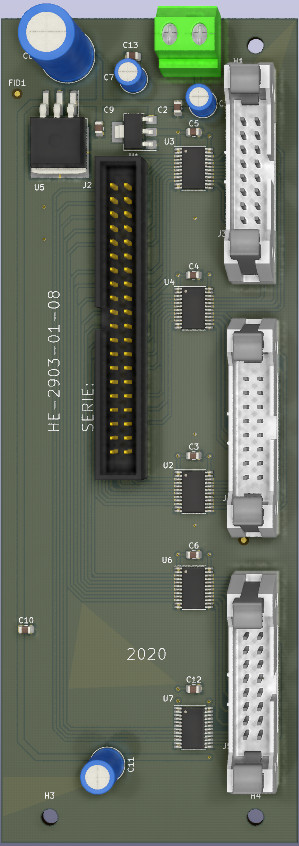
\includegraphics[scale=0.5]{Figures/renderpcbfrontaldistribuccion.jpg} 
	\caption{Vista frontal del PCB de distribución.}
	\label{fig:pcbrenderdistribuccionfrontal}
\end{figure}

\begin{figure}[htpb]
	\centering
    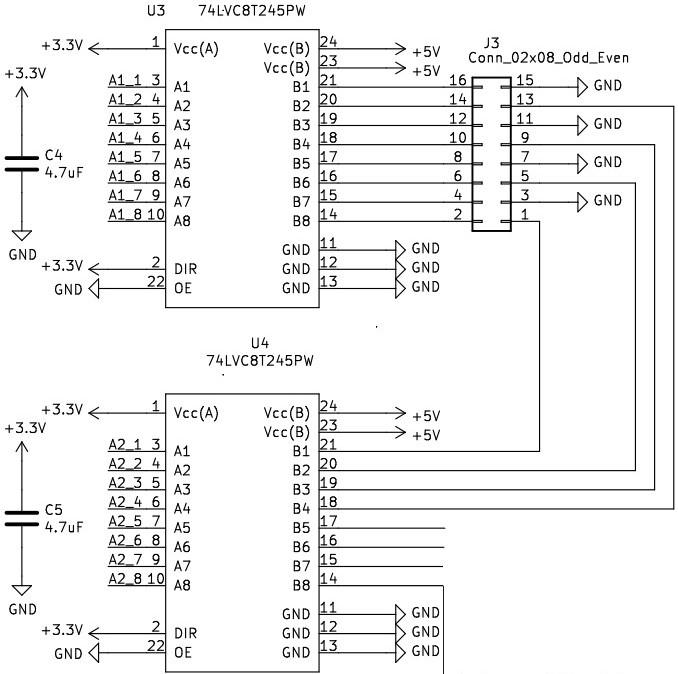
\includegraphics[scale=0.5]{Figures/circuitodistribucion.jpg} 
	\caption{Circuito de una salida de la PCB de distribución.}
	\label{fig:circuitodistribucion}
\end{figure}

\begin{figure}[htpb]
	\centering
    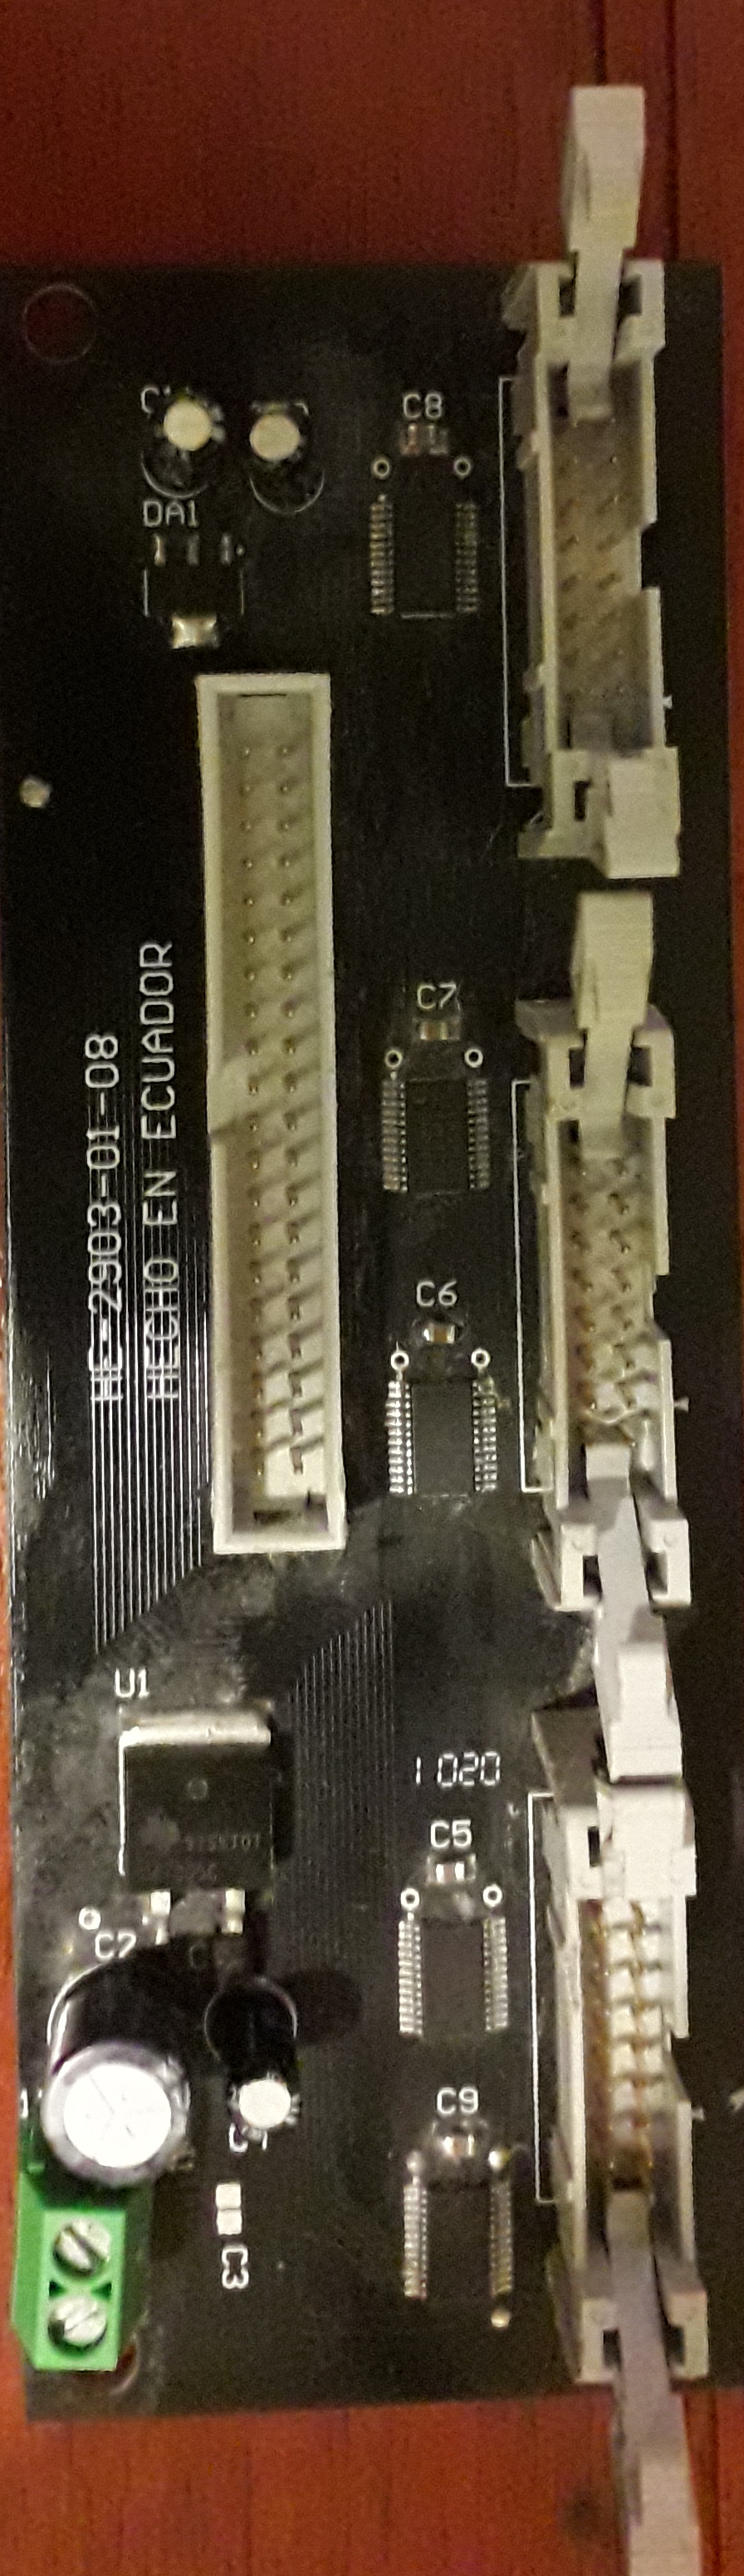
\includegraphics[scale=0.1]{Figures/pcbdistri.jpg} 
	\caption{Foto PCB de distribución.}
	\label{fig:fotopcbdistri}
\end{figure}

\section{ Diseño del firmware}
El firmware fue escrito en lenguaje C. El firmware es administrado por el sistema operativo Linux. El firmware es ejecutado por un servicio. El servicio es administrado por SYSTEMD. Las imágenes son almacenadas  dentro de la carpeta compartida mediante SAMBA. 

Los archivos de configuración son almacenados en la carpeta de configuraciones en varios archivos CSV. En la figura \ref{fig:agendacsv} se muestra el archivo AGENDA.csv. El archivo AGENDA.csv contiene el numero de imagen y el tiempo en segundos que se debe mostrar la imagen en la pantalla.

\begin{figure}[htpb]
	\centering
    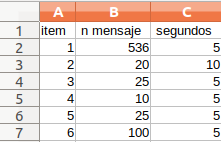
\includegraphics[scale=0.7]{Figures/Agenda.png} 
	\caption{Archivo AGENDA.csv.}
	\label{fig:agendacsv}
\end{figure}


El archivo CONFIGURACION.csv contiene la ultima configuración de las banderas clima y reloj. Esta configuración se usa al iniciar el sistema.

El archivo IPBASE.csv contiene la dirección IP de la central de control.

En la figura \ref{fig:offlinecsv} se muestra el archivo OFFLINE.csv. El archivo OFFLINE.csv contiene el numero de imagen y el tiempo en segundos que se debe mostrar la imagen en la pantalla cuando la pantalla pierde conexión con la central de control.

\begin{figure}[htpb]
	\centering
	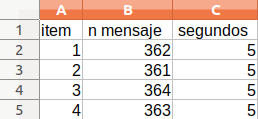
\includegraphics[scale=0.7]{Figures/offline.png} 
	\caption{Archivo OFFLINE.csv.}
	\label{fig:offlinecsv}
\end{figure}
EL archivo FIFO llamado myfifo se usa para interactuar con otros programas que se encuentran en el sistema por medio de este se puede actualizar las imágenes que se muestran en pantalla.


Las tareas que realiza el firmware son:
\begin{itemize}
\item Procesar la comunicación UDP.
\item Funcionar de acuerdo a la programación preestablecida en los archivos de configuración.
\item Desplegar imágenes previamente almacenadas en la memoria SD.  
\item Desplegar un conjunto de imágenes diferentes si se pierde la conexión con la central de control.
\item Generar y mostrar un reloj en la pantalla en función de la configuración.
\item Mostrar datos relevantes del clima en la pantalla en función de la configuración.
\item Mostrar tiempos de viaje en la pantalla en función de la configuración.
\item Interacción con otros programas mediante archivos FIFO.
\item Mostrar mensajes de emergencia que se muestran solo por un tiempo definido.
\item Reorganizar la imagen leída de la memoria SD y almacenarla en la memoria compartida con el FPGA.
\item Mostrar actualizaciones de las tareas realizadas en la consola.
\end{itemize}

La solución alcanzada consta de cuatro hilos. En las figuras \ref{fig: hiloprincipal1} y \ref{fig: hiloprincipal2} muestran el diagrama de flujo del hilo principal del firmware. 

La comunicación con la estación remota es manejada por el hilo de comunicaciones. Los diagramas de flujo de el hilo de comunicación se muestran en las figuras \ref{fig: hilocomparte1}, \ref{fig: hilocomparte2} y \ref{fig: hilocomparte3}.

La interacción con otros programas es manejada por el hilo de FIFO. El diagrama de flujo se muestra en la figura \ref{fig: hilofifo}.

El último hilo comprueba la comunicación con la estación remota y actualiza la bandera comunicación.

\begin{figure}[htpb]
	\centering
	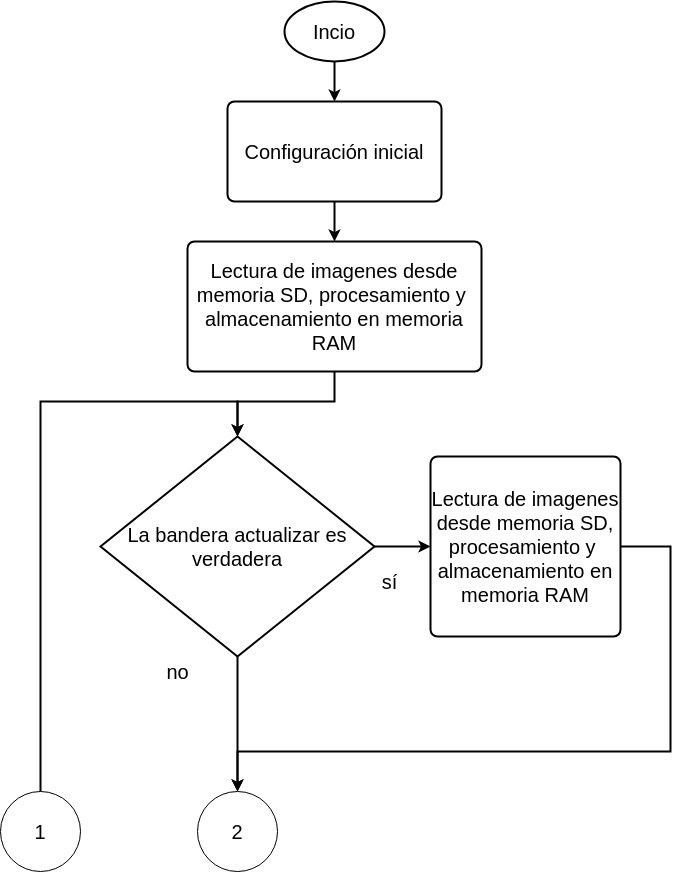
\includegraphics[scale=0.6]{Figures/hilo1parte1.jpg} 
	\caption{Diagrama de flujo del hilo principal parte uno.}
	\label{fig: hiloprincipal1}
\end{figure}
\begin{figure}[htpb]
	\centering
	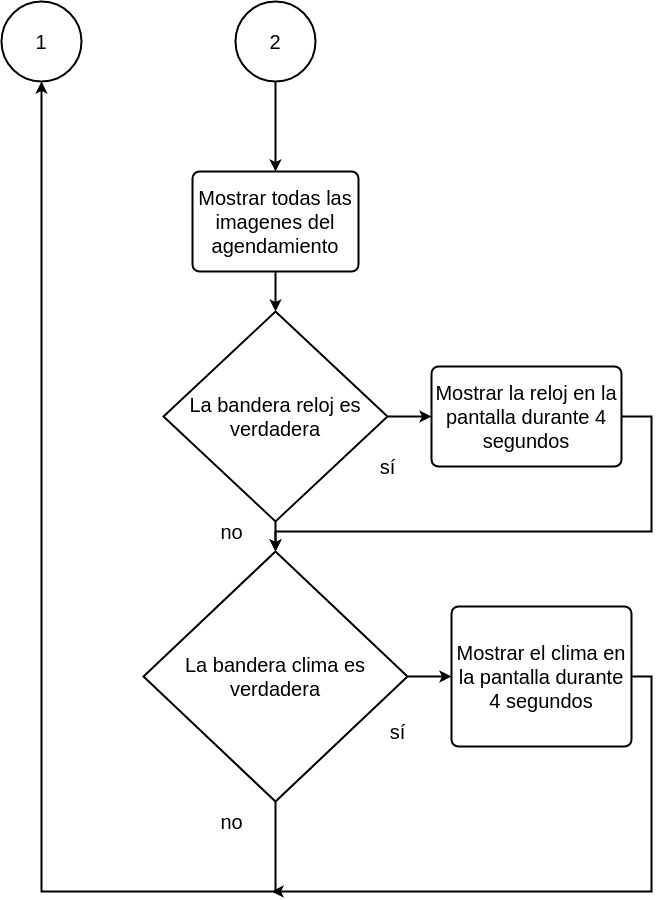
\includegraphics[scale=0.6]{Figures/hilo1parte2.jpg} 
	\caption{Diagrama de flujo del hilo principal parte dos.}
	\label{fig: hiloprincipal2}
\end{figure}


\begin{figure}[htpb]
	\centering
	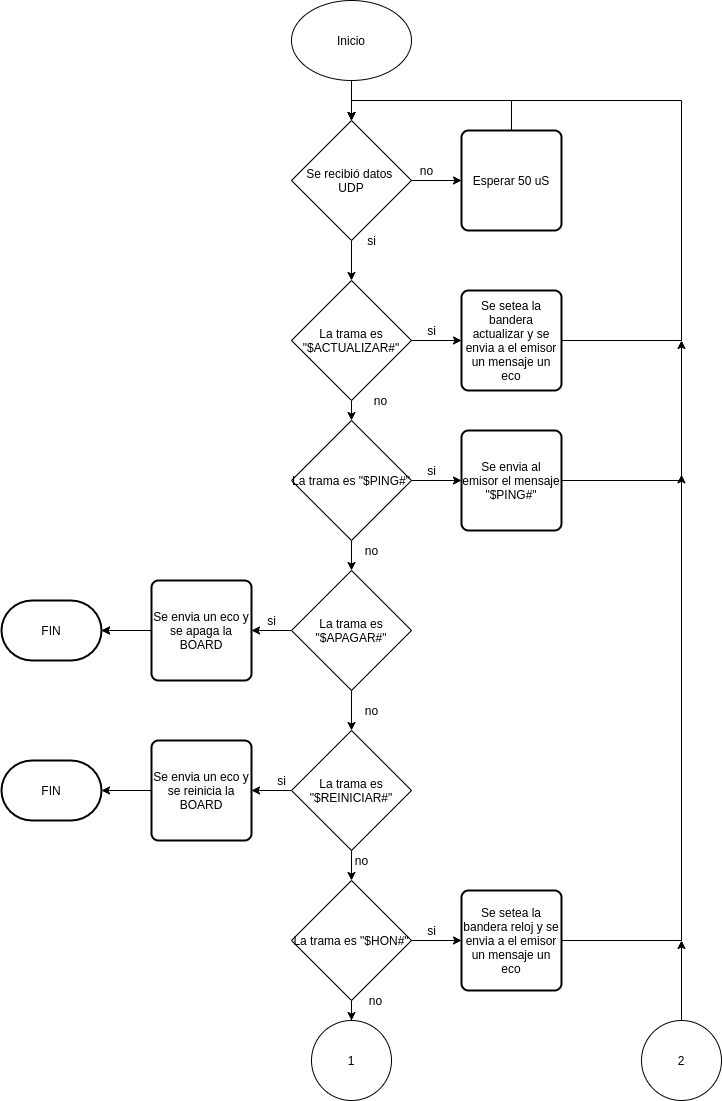
\includegraphics[scale=0.6]{Figures/hilo2parte1.jpg}  
	\caption{Diagrama de flujo del hilo de comunicaciones parte uno.}
	\label{fig: hilocomparte1}
\end{figure}

\begin{figure}[htpb]
	\centering
	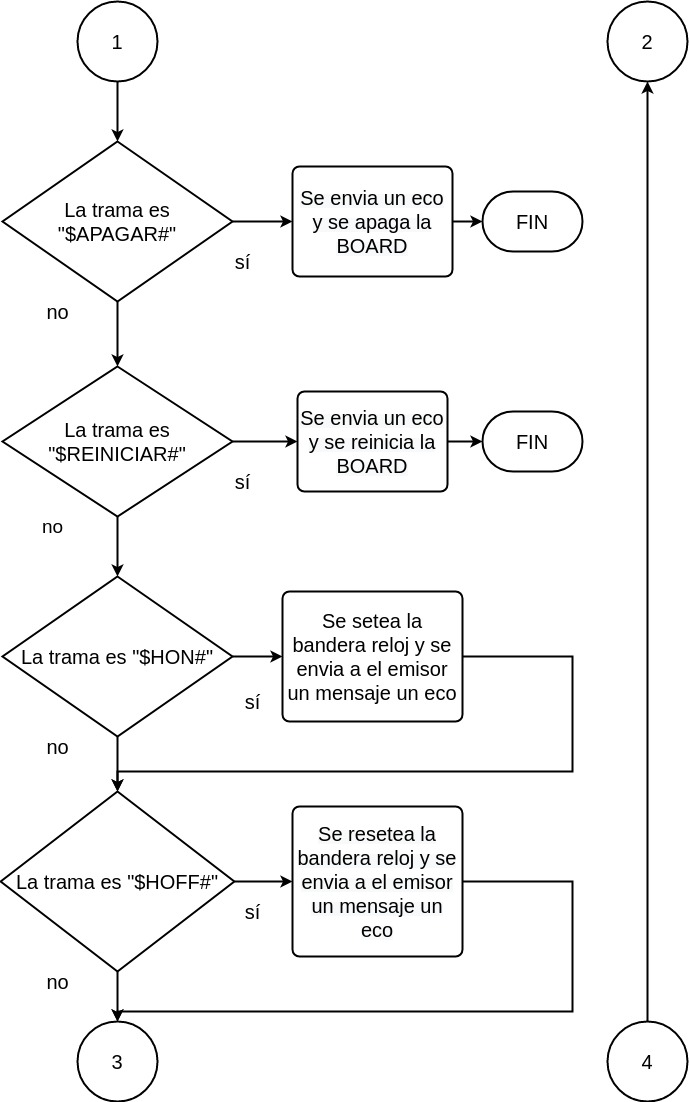
\includegraphics[scale=0.6]{Figures/hilo2parte2.jpg} 
	\caption{Diagrama de flujo del hilo de comunicaciones parte dos.}
	\label{fig: hilocomparte2}
\end{figure}

\begin{figure}[htpb]
	\centering
	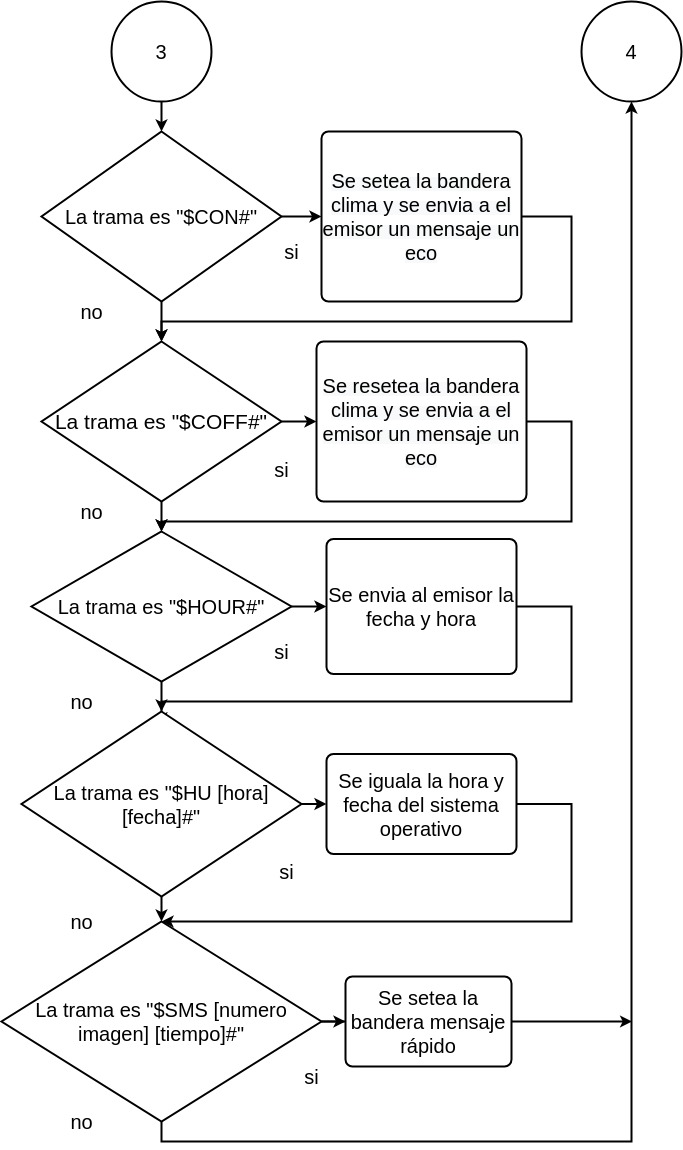
\includegraphics[scale=0.6]{Figures/hilo2parte3.jpg} 
	\caption{Diagrama de flujo del hilo de comunicaciones parte tres.}
	\label{fig: hilocomparte3}
\end{figure}


\begin{figure}[htpb]
	\centering
	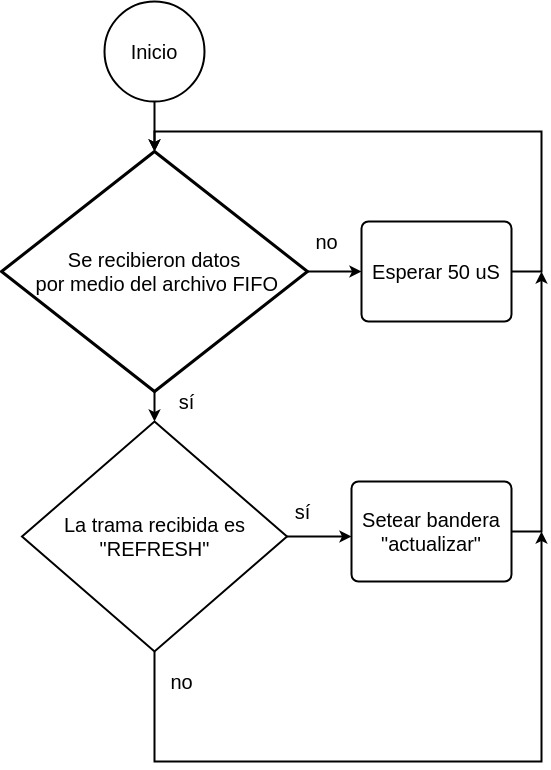
\includegraphics[scale=0.7]{Figures/hilo3.jpg} 
	\caption{Diagrama de flujo del hilo interacción con programas externos.}
	\label{fig: hilofifo}
\end{figure}
\pagebreak

\section{ Diseño de lógica programable}
Para controlar las matrices de la pantalla LED se deben realizar varios procesos simultáneos ademas de controlar una gran cantidad de salidas GPIO. Por esta razón se decidió utilizar el FPGA para controlar la matriz de LEDs.
El FPGA realiza las siguientes tareas:
\begin{itemize}
\item Leer los bytes ya procesados por el firmware de la memoria compartida con el procesador. 
\item Controlar simultáneamente seis filas de matrices de LEDs.
\item Apagado controlado de la matriz de LEDs por medio de una señal Lightweigth HPS-to-FPGA.
\end{itemize}

Mediante la herramienta de diseño de QUARTUS (PLATFORM DESIGNER) se interconectaron los módulos como se muestran en la siguiente figura \ref{fig: platform}. Un resumen de los módulos se muestra a continuación:
\begin{itemize}
\item El módulo System\_PLL tiene la función de generar dos relojes un de 100 MHz para el procesador y un reloj de 50 MHz para el FPGA.
\item El módulo onchip\_ram es una memoria ram dual asincrónica. La memoria es compartida por el FPGA y el procesador. 
\item El módulo pio\_0 es la comunicación Lightweigth HPS-to-FPGA. 
\item El módulo ARM\_9\_HPS es el procesador. 
\end{itemize}

El FPGA funciona con una maquina de estados finita. La maquina de estados se muestra en la figura \ref{fig: diagrama estados}. Debido a un error en el diseño del la PCB matriz de LEDs se deben apagar todos los LEDs para cambiar la imagen. El procesador señala el cambio de imagen mediante la comunicación Lightweigth HPS-to-FPGA pio\_0.

 



\begin{figure}[htpb]
	\centering
	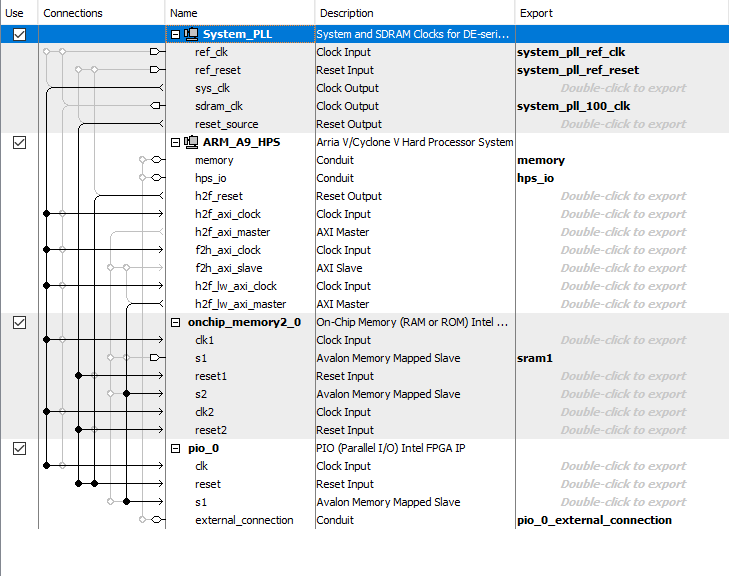
\includegraphics[scale=0.8]{Figures/platformdesigner.png} 
	\caption{Configuración del PLATFORM DESIGNER.}
	\label{fig: platform}
\end{figure}


\begin{figure}[htpb]
	\centering
	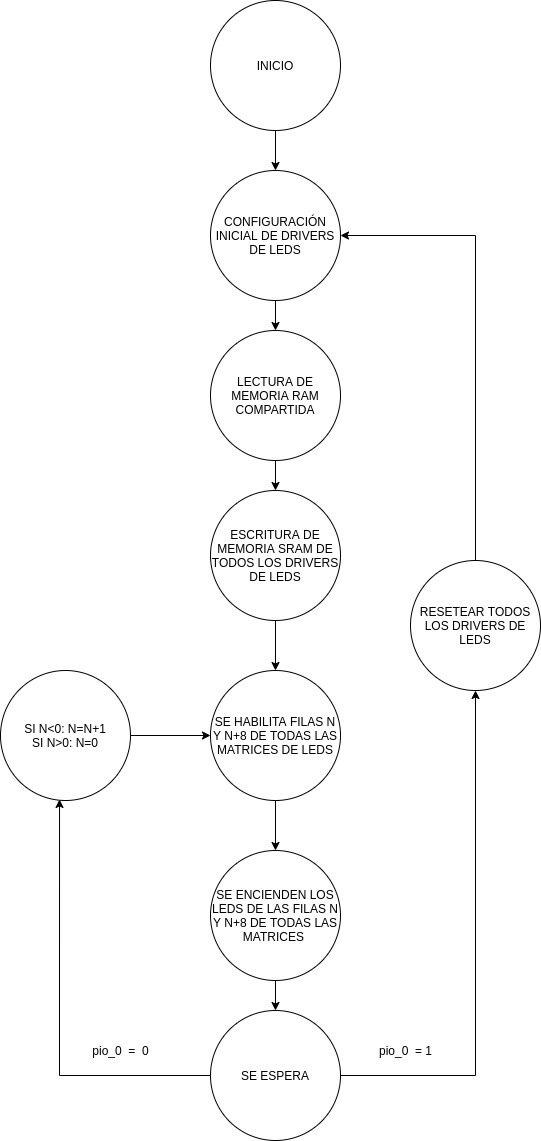
\includegraphics[scale=0.6]{Figures/maquinaestados.jpg} 
	\caption{Diagrama de maquina de estados del FPGA.}
	\label{fig: diagrama estados}
\end{figure}







